\chapter{Understanding Rainfall Rate and Flood Occurrences}

In this chapter, one of the potential explanatory variable for the flood occurrences in Jakarta, which is the rainfall rate, will be investigated. \\

\section{Rainfall Rate Throughout the Year 2013 Until 2017}

The rainfall rate data in a csv file format is obtained from the BPS website and this data is open for anybody to use it. The csv file contains monthly rainfall rate from the year of 2009 until 2017. However, to accommodate the available flood occurrences data, the rainfall rate that will be considered are the rate in the span of 2013 until 2017. Figure \ref{fig=rainfall.png} shows the trends of the rainfall rate in Jakarta throughout 2013 until 2017.\\

\begin{figure}
\begin{center}
\graphicspath{ {./Pict/} }
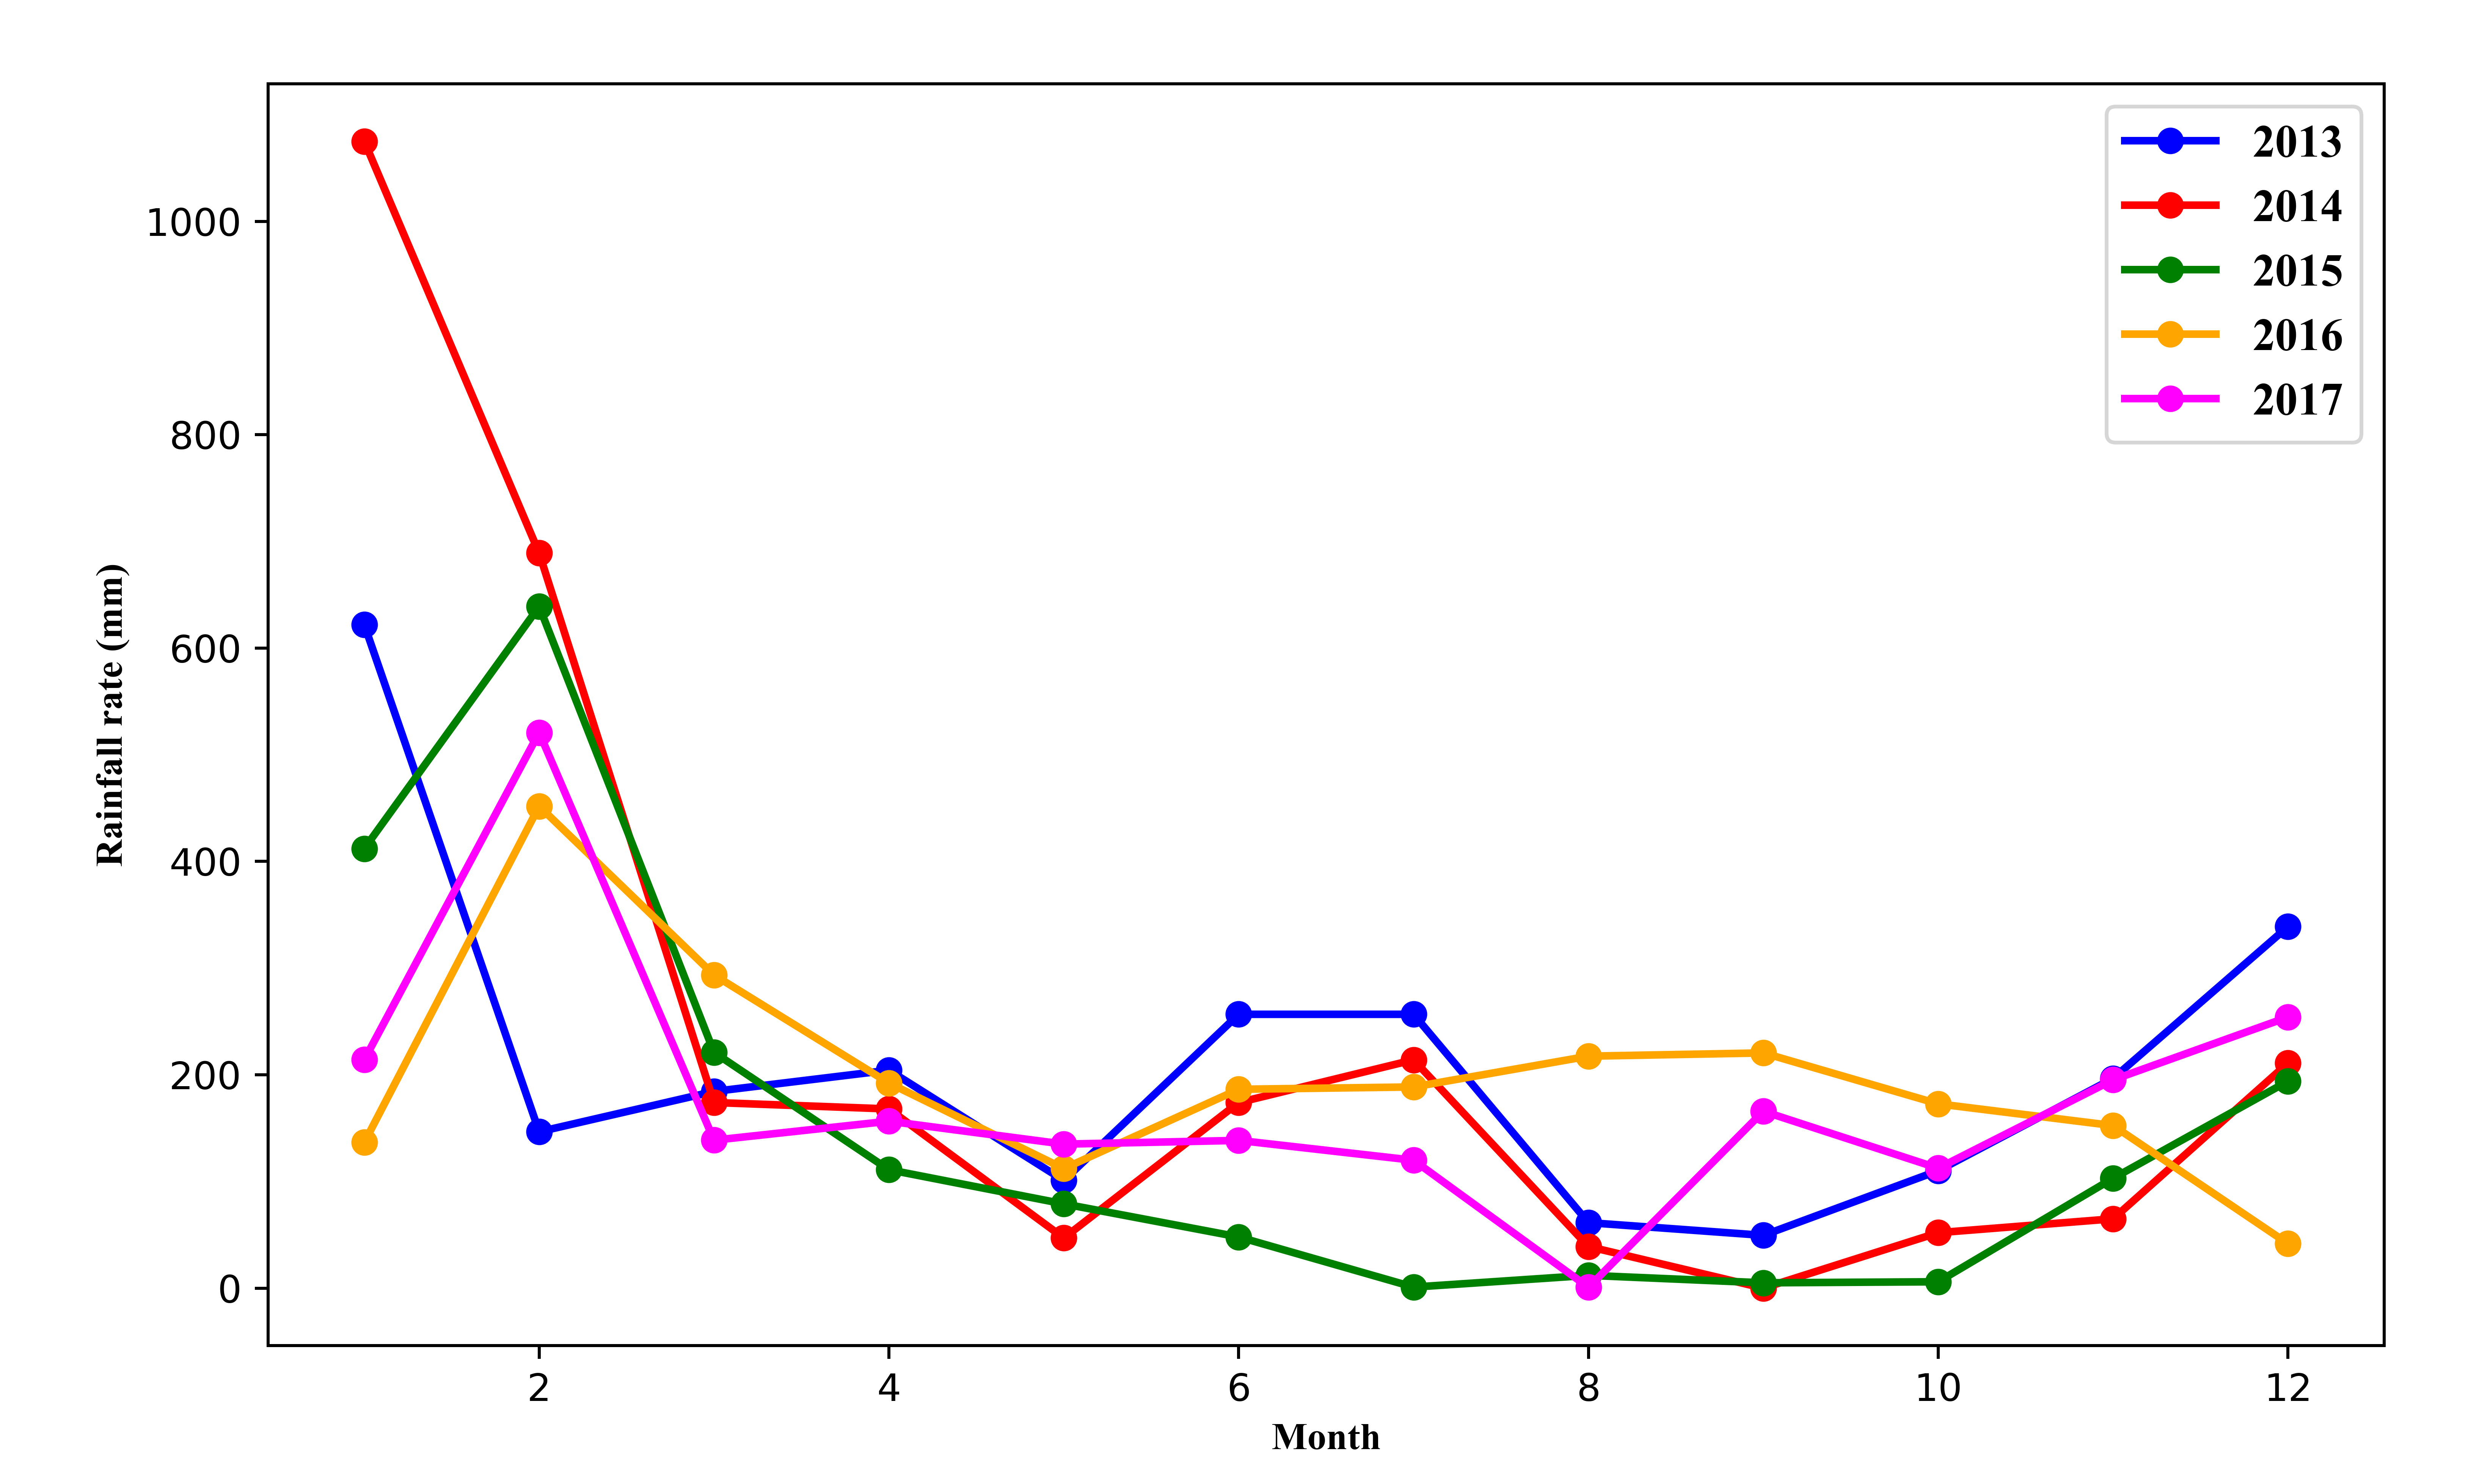
\includegraphics[scale=0.15]{rainfall.png}
\caption{Rainfall rate in Jakarta throughout 2013-2017}\label{fig=rainfall.png}
\end{center}
\end{figure}

\noindent
From Figure \ref{fig=rainfall.png}, it can be seen that there are certain patterns regarding the rainfall rate in any given year. In general, the rainfall rate reach its highest in January and February. Then, from March and the following month the rate is gradually dipping until it  reaches its lowest point between the month of August until October before it starts to increase again from November and so on. \\

\noindent
However, before drawing any conclusion from Figure \ref{fig=rainfall.png}, the trends regarding the flood occurrences in Jakarta throughout 2013 until 2017 needs to be investigated first. This is necessary to check whether there might be a correlation between flood occurrences and rainfall rate.

\section{Flood Occurrences Throughout the Year 2013 Until 2017}

Before visualizing the trend regarding the flood occurrence in Jakarta, first a variable to quantify the occurrence of floods needs to be defined. In order to quantify the flood occurrence, the number of sub-districts that have been affected by floods in any given month throughout 2013 until 2017 is investigated. Figure \ref{fig=flood.png} shows the amount of sub-districts in Jakarta that have been affected by floods from 2013 until 2017.\\

\begin{figure}
\begin{center}
\graphicspath{ {./Pict/} }
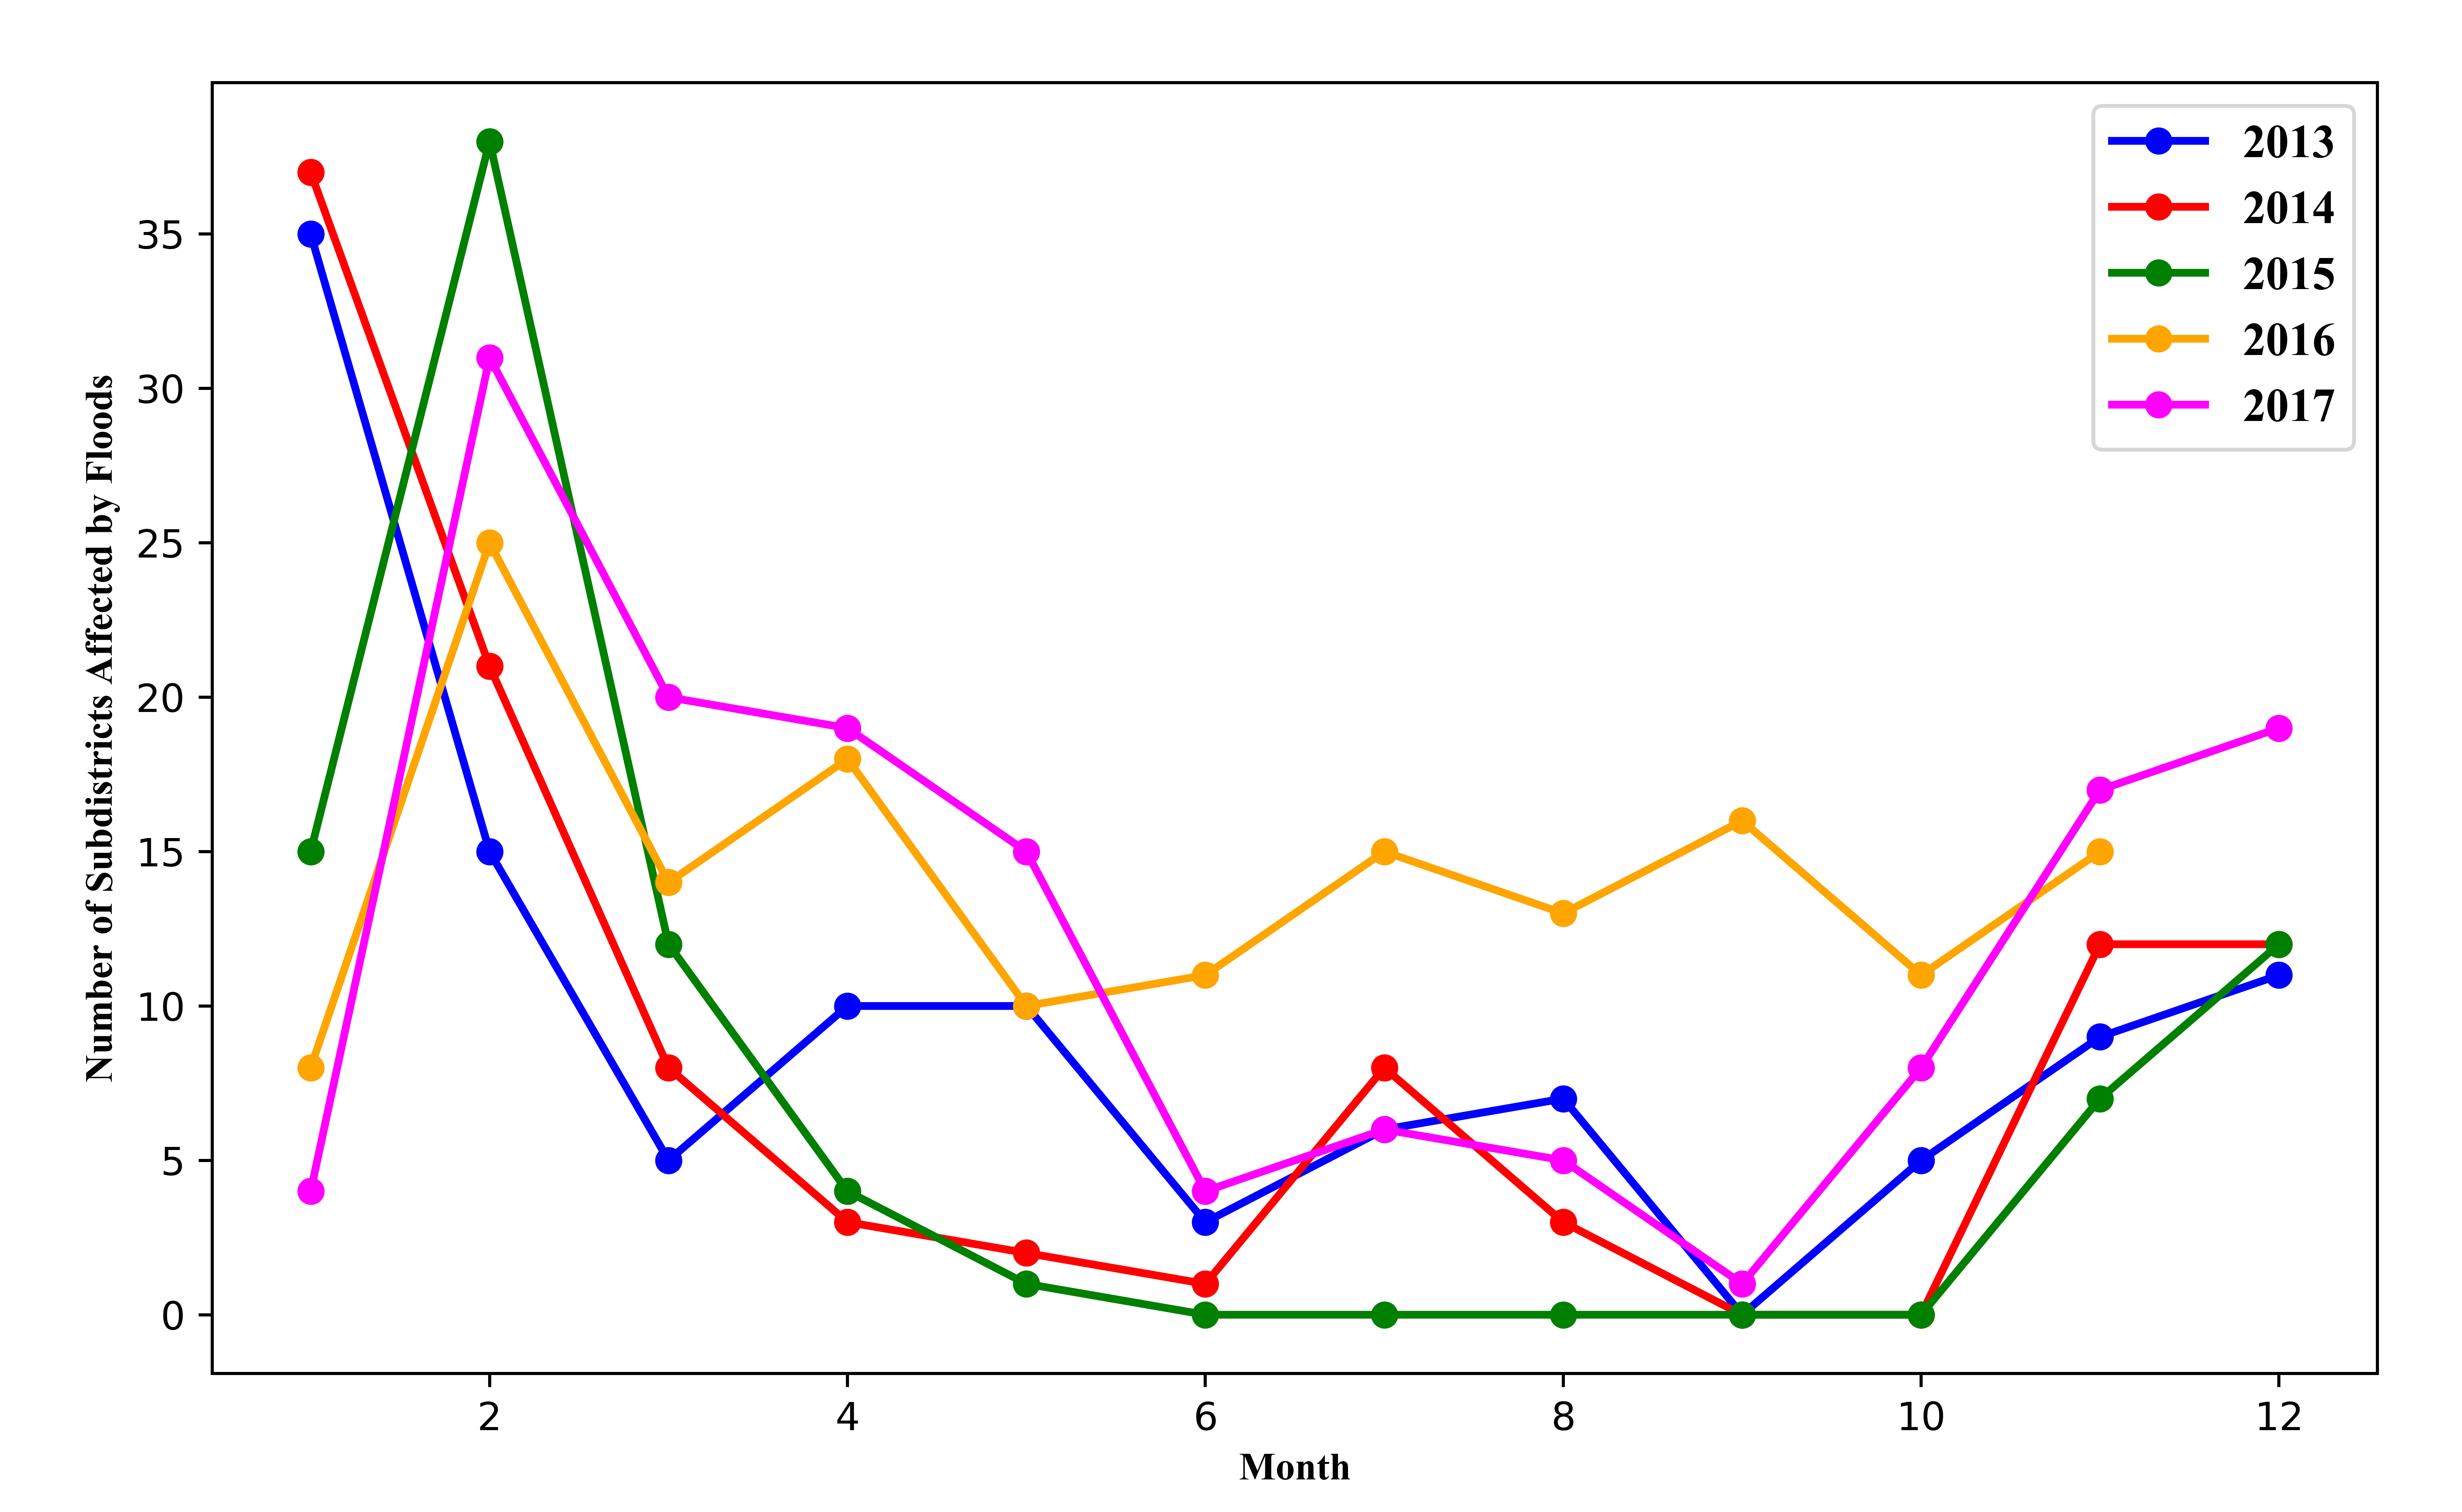
\includegraphics[scale=0.15]{flood.png}
\caption{Flood occurrences in Jakarta throughout 2013-2017}\label{fig=flood.png}
\end{center}
\end{figure}

\noindent
From Figure \ref{fig=flood.png}, it can be concluded that there are similar patterns of flood occurrences and rainfall rate. The flood case in Jakarta reach its highest during January and February, in which at least five districts affected by floods. Then, starting from March and the following month the flood occurrence is decreasing until reaches its lowest starting in June until October before it starts to increase again on November and so on.\\

\noindent
Because of the similarity of patterns between rainfall rate and flood occurrences, hence it can be concluded that there are positive correlation between one another. However, the direct correlation between these two variables will be discussed in more detail in the next chapter. \\

\noindent
From the Figure \ref{fig=rainfall.png} and Figure  \ref{fig=flood.png}, a suggestion can be made to the authorities and the government regarding the best period of time in a year to prepare some mitigation measurements. Since the flood occurrences and rainfall reach their lowest in around May until October, then it can be suggested that between the month of May until October are the best period of time to do some precautionary and mitigation measurements of the floods.\\


